%!TEX root = ../../../adrien_gomar_phd.tex
\paragraph{Using the advection equation model problem}

A pure harmonic signal is imposed at the left boundary condition
of the linear advection equation toy problem presented in Sec.~\ref{sec:toy_convection}:
\begin{equation}
   u_l (t) = 1 + \sin \left(2 \pi f t\right).
\end{equation}
The minimal condition number
$\kappa(E) = 1$ is obtained with evenly spaced time instances.
In fact, as the injected function is mono-frequential, 
the theoretical lower of the condition number is obtained by using evenly
spaced time instances.
The time instances of the harmonic balance
computations are chosen to reach varying condition numbers
such that $1 \leq \kappa (E) \leq 10$.  

As shown in the previous section, the condition number 
can, by definition, amplify the error made
on the iterative resolution of the linear advection equation.
This is illustrated in Fig.~\ref{fig:condition_number_local_amp} which 
shows the evolution of the results with a varying condition number.
The amplitude of the
sinusoidal function is either under or over-estimated when
$\kappa (E) \neq 1$. However, 
the higher the condition number, the worse the accuracy in capturing
the amplitude of the injected function. Moreover, when $\kappa(E) \geq 6$,
the shape of the solution is even inverted which would lead to
bad conclusions if analyzed as it.
\begin{figure}[htbp]
  \centering
  \includegraphics*[width=0.50\textwidth]{condition_number_local_amp.pdf}
  \caption{Linear advection of a sinusoidal function: numerical steady-state 
  solutions at $t=0$ for varying condition number.}
  \label{fig:condition_number_local_amp}
\end{figure}

\paragraph{Using the channel flow toy problem}
The previous example was based on the advection equation which
has the good property of having a analytical solution to 
analyze the results. The results show that the harmonic
balance solutions are very sensitive to the condition number.
To further analyze the condition number issue,
the unsteady channel flow toy problem
(see Sec.~\ref{sec:toy_channel}) is computed with a single
frequency oscillating back-pressure 
at the outlet: $f_1 = 3$~Hz, the second
frequency having a zero amplitude: $a_2= 0$:
\begin{equation}
   P_{outlet} (t) = P_m \left[ 1 + a_1 \sin \left(2 \pi f_1 t\right) \right].
\end{equation}
This helps understanding the behavior of the HB source term
withing the Navier--Stokes equations framework.

As the oscillating back-pressure is composed of only one frequency,
it is mono-frequential.
Thus, by using evenly-space time instances, the condition
number of the source term is unity $\kappa (E) = 1$. 
To highlight the issue related to the condition number,
the time instances are chosen to reach varying condition numbers
such that $1 \leq \kappa (E) \leq 3.43$.  
Two frequencies are
specified for the HB computation: $f_1$ and its first harmonic
$2f_1$. 


\begin{figure}[htb!]
  \centering
  \subfigure[$a_1 = 0.01$]{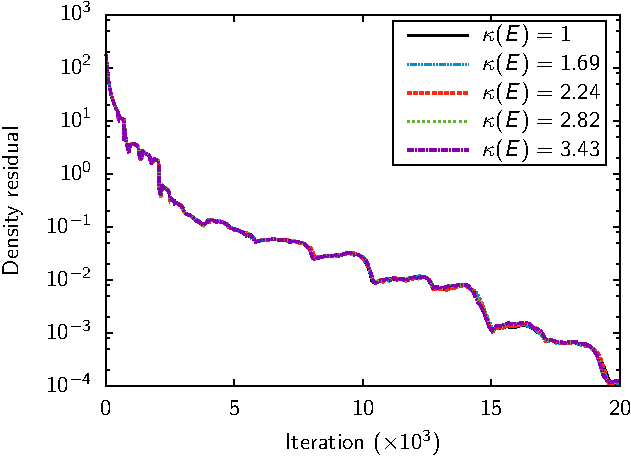
\includegraphics[width=.45\textwidth]{CANAL2_RESIDUAL_VS_CONDITIONNING_AMP001_PPT.pdf}}
  \subfigure[$a_1 = 0.05$]{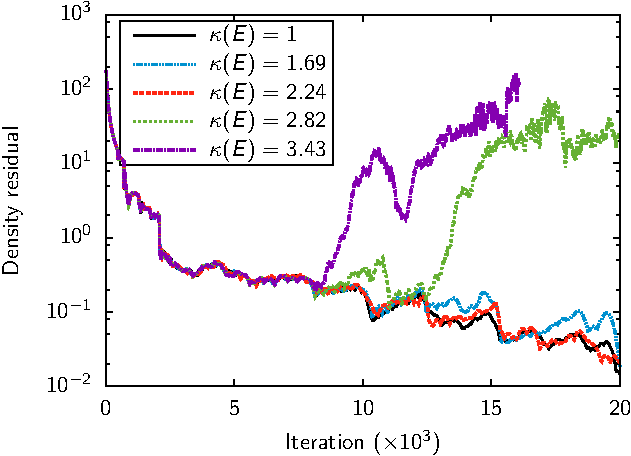
\includegraphics[width=.45\textwidth]{CANAL2_RESIDUAL_VS_CONDITIONNING_AMP005_PPT.pdf}}
  \caption{Relation between the condition number $\kappa (E)$ and the convergence of the solution.}
  \label{fig:canal_residual_vs_conditionning}
\end{figure}
The results in Fig.~\ref{fig:canal_residual_vs_conditionning} show that
for a condition number $\kappa (E) \geq 2.24$ and wave input amplitude
$a_1 = 0.05$, the computation diverges. However, the computations with
the same condition numbers but a smaller input amplitude $a_1 = 0.01$
converge. In fact, the condition number amplifies the errors made
during the iterative process. When the input waves have a smaller
amplitude, the iterative errors are slighter.

In our case, the amplitude of the computed unsteady phenomena can not
be \emph{a priori} known. Therefore, the section below will be dedicated to
the development of algorithms to minimize the condition number.
